%---------------Template for figures in TikZ---------------%
%----can be used for either single or multiple diagrams----%
\documentclass{standalone}
%\documentclass[a4paper]{article}
\usepackage{tikz}
\pagestyle{empty}
\usepackage[utf8]{inputenc}
\usepackage[english]{babel}
\usepackage{pgfplots}
\usepackage{tikz}
\usetikzlibrary{plotmarks}
\usetikzlibrary{spy}
\usepackage{amsmath}
\usepackage{textcomp}
\usepackage{gensymb}
\usepackage{color}
\DeclareMathOperator\arsinh{arsinh}
\tikzset{dashdot/.style={dash pattern=on 4pt off 2pt on 1pt off 2pt}}
\tikzset{dashed/.style={dash pattern=on 4pt off 2pt}}
%\pgfplotsset{compat=1.9}
\pgfdeclarelayer{background}
\pgfsetlayers{background,main}
\usetikzlibrary{shapes,arrows,shadows,positioning}
\usetikzlibrary{backgrounds}



\tikzset{
  font={\fontsize{8pt}{12}\selectfont}}
\begin{document}

%\hspace{-1.5cm}





\begin{tikzpicture}
 	

\node at (-3,9) {wild-type};
\node at (-5.5,9) {A};
\node[inner sep=0pt] (russell) at (-3,7)
    {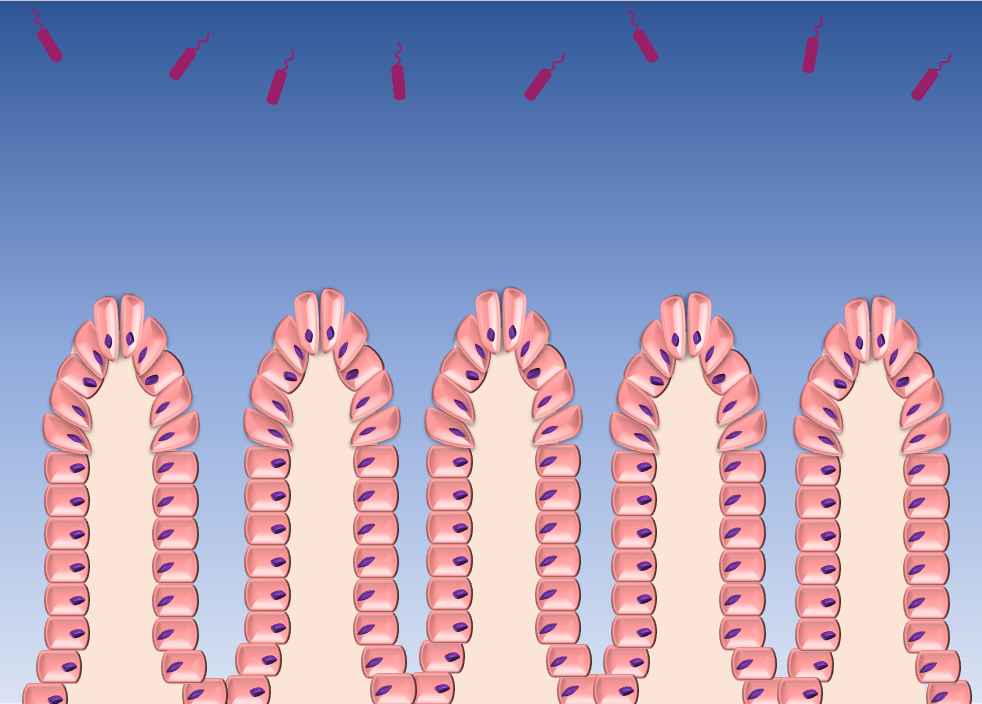
\includegraphics[width=.4\textwidth]{in-n1.png}};   	
%-=-=-=-=-=-=-=-=-=-=-=-=-=-=-=-=-=-=-=-=-=-=-=-=-=-=-=-=-=-=

\node at (3,9) {MyD88 knockout};
\node at (0.5,9) {B};
\node[inner sep=0pt] (russell) at (3,7)
    {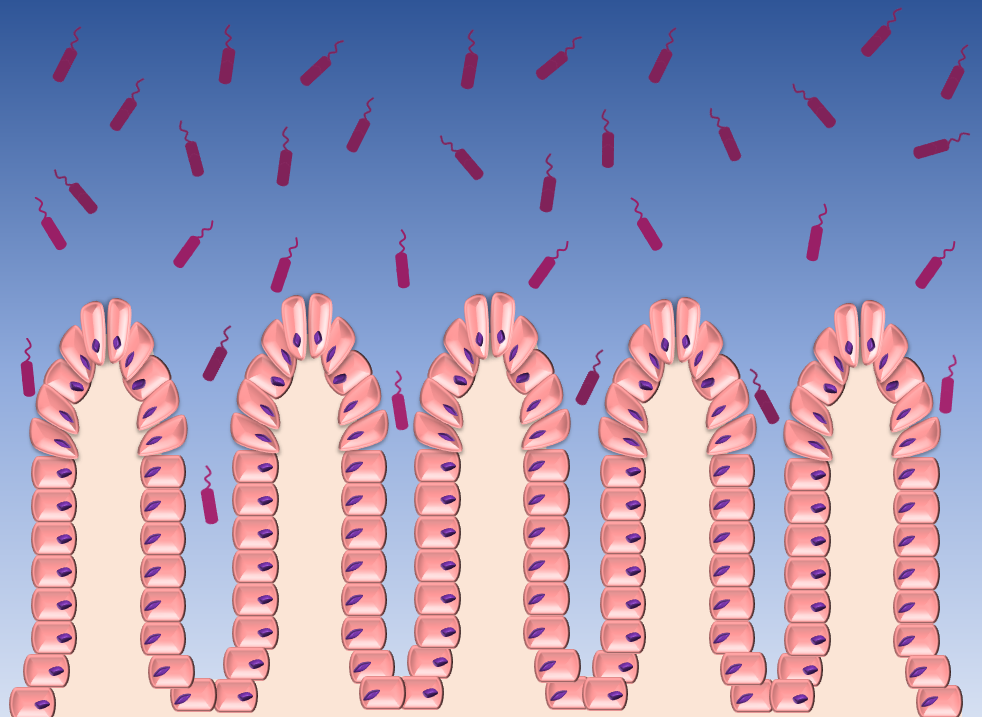
\includegraphics[width=.4\textwidth]{in-n2.png}};   	
%-=-=-=-=-=-=-=-=-=-=-=-=-=-=-=-=-=-=-=-=-=-=-=-=-=-=-=-=-=-=


\node at (-5.5,4.5) {C};
\node[inner sep=0pt] (russell) at (-3,1.)
    {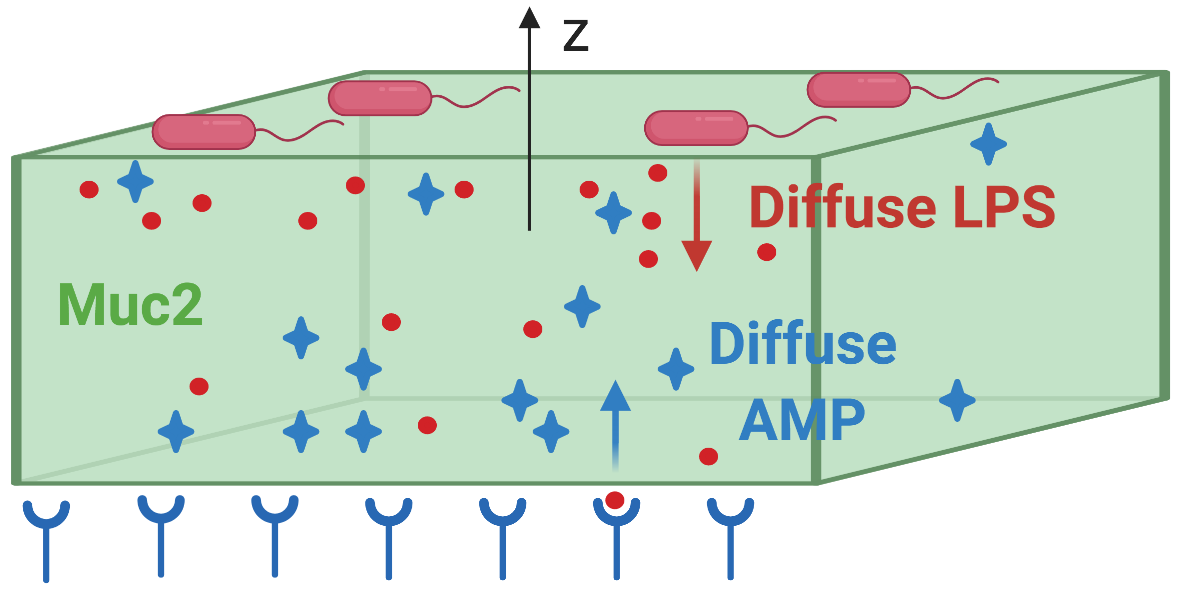
\includegraphics[width=.45\textwidth]{model.png}};   	
\node at (-1.2,-0.2) {LPS receptors};

%-=-=-=-=-=-=-=-=-=-=-=-=-=-=-=-=-=-=-=-=-=-=-=-=-=-=-=-=-=-=

\node at (0.5,4.5) {D};
\node[inner sep=0pt] (russell) at (2.75,2.2)
    {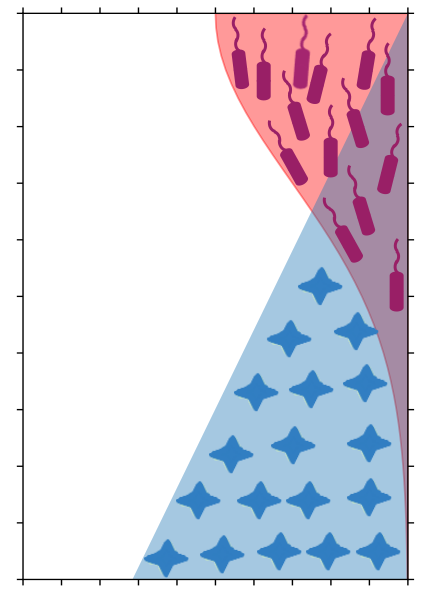
\includegraphics[width=4.cm, height=4.2cm]{svg2.png}};   	
\node at (2.9,-0.3) {Local concentrations};
\node [rotate=90] at (5.2,2.3) {Distance from the interface (z)};
\node [rotate=90] at (4.8,0.25) {0};
\node [rotate=90] at (4.8,4.2) {1};
\node [rotate=0] at (2.45,3.8) {$\lambda_1$};
\draw[thick, <->,rotate=90] (3.,-2.65) -- (4.2,-2.65);

\node [rotate=0] at (4.6,0.1) {0};
\node [rotate=0] at (0.95,0.1) {1};
\node [rotate=0] at (2.,0.1) {$a_0$};
\node [rotate=0] at (2.9,4.4) {$b_{M1}$};

\node[inner sep=0pt,opacity=0.2] (russell) at (2.8,-0.2)
    {
\includegraphics[width=.35\textwidth]{gut.png}};  

%-=-=-=-=-=-=-=-=-=-=-=-=-=-=-=-=-=-=-=-=-=-=-=-=-=-=-=-=-=-=


\node[inner sep=0pt] (russell) at (-1.2,3.4)
    {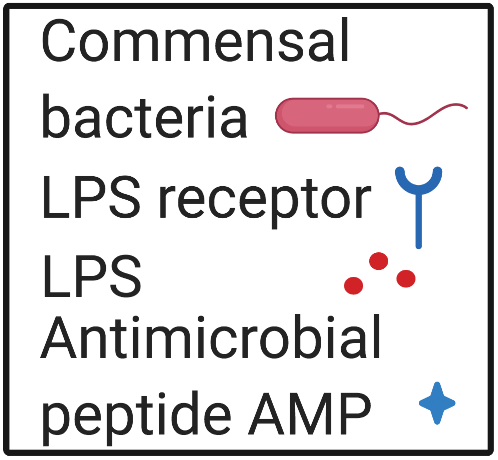
\includegraphics[width=.15\textwidth]{legend.png}};   	

\node [single arrow,black,draw,inner sep=.0cm,minimum height=.7cm, single arrow head extend=0.05cm,anchor=west,fill=black,rotate=0] at (-6,6) (blk){ };    
\node [rotate=0] at (-6.2,6.2) {Epithelium}; 


\node [single arrow,black,draw,inner sep=.0cm,minimum height=.7cm, single arrow head extend=0.05cm,anchor=west,fill=black,rotate=0] at (-6,8.4) (blk){ };    
\node [rotate=0] at (-5.9,8.6) {Lumen}; 


\node [single arrow,black,draw,inner sep=.0cm,minimum height=.7cm, single arrow head extend=0.05cm,anchor=west,fill=black,rotate=0] at (-6,7.4) (blk){ };    
\node [rotate=0] at (-5.9,7.6) {Mucus}; 


\end{tikzpicture}


\end{document}


